\documentclass{standalone}
\usepackage{pgfplots}\pgfplotsset{compat=1.17}
\begin{document}
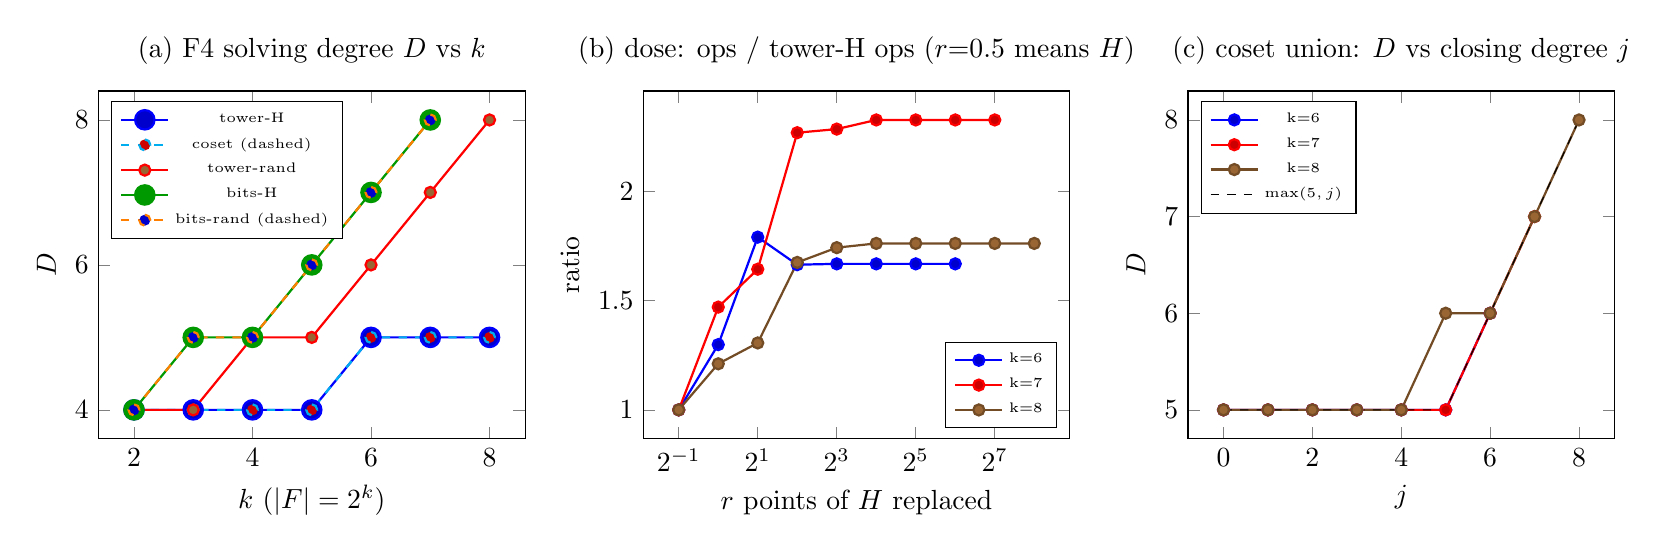
\begin{tikzpicture}
\begin{axis}[name=a,title={(a) F4 solving degree $D$ vs $k$},xlabel={$k$ ($|F|=2^k$)},ylabel={$D$},legend pos=north west,legend style={font=\tiny},width=7cm,height=6cm]
\addplot+[mark=*,thick,blue,mark size=3.5pt] coordinates {(2,4)(3,4)(4,4)(5,4)(6,5)(7,5)(8,5)}; \addlegendentry{tower-H}
\addplot+[mark=*,thick,cyan,dashed] coordinates {(2,4)(3,4)(4,4)(5,4)(6,5)(7,5)(8,5)}; \addlegendentry{coset (dashed)}
\addplot+[mark=*,thick,red] coordinates {(2,4)(3,4)(4,5)(5,5)(6,6)(7,7)(8,8)}; \addlegendentry{tower-rand}
\addplot+[mark=*,thick,green!60!black,mark size=3.5pt] coordinates {(2,4)(3,5)(4,5)(5,6)(6,7)(7,8)}; \addlegendentry{bits-H}
\addplot+[mark=*,thick,orange,dashed] coordinates {(2,4)(3,5)(4,5)(5,6)(6,7)(7,8)}; \addlegendentry{bits-rand (dashed)}
\end{axis}
\begin{axis}[name=b,at={(a.east)},anchor=west,xshift=1.5cm,xmode=log,log basis x=2,title={(b) dose: ops / tower-H ops ($r{=}0.5$ means $H$)},xlabel={$r$ points of $H$ replaced},ylabel={ratio},legend pos=south east,legend style={font=\tiny},width=7cm,height=6cm]
\addplot+[mark=*,thick,] coordinates {(0.5,1)(1,1.2988789842895183)(2,1.7911354591518427)(4,1.6649390546172336)(8,1.6687213869719228)(16,1.6687213869719228)(32,1.6687213869719228)(64,1.6687213869719228)}; \addlegendentry{k=6}
\addplot+[mark=*,thick,] coordinates {(0.5,1)(1,1.4706425971422583)(2,1.644168392672498)(4,2.2694142962614134)(8,2.285968940793037)(16,2.327877579864677)(32,2.327877579864677)(64,2.327877579864677)(128,2.327877579864677)}; \addlegendentry{k=7}
\addplot+[mark=*,thick,] coordinates {(0.5,1)(1,1.2110529202723308)(2,1.3065146786043365)(4,1.6753321975965716)(8,1.7429479046520342)(16,1.762390835429981)(32,1.762390835429981)(64,1.762390835429981)(128,1.762390835429981)(256,1.762390835429981)}; \addlegendentry{k=8}
\end{axis}
\begin{axis}[name=c,at={(b.east)},anchor=west,xshift=1.5cm,title={(c) coset union: $D$ vs closing degree $j$},xlabel={$j$},ylabel={$D$},legend pos=north west,legend style={font=\tiny},width=7cm,height=6cm]
\addplot+[mark=*,thick,] coordinates {(0,5)(1,5)(2,5)(3,5)(4,5)(5,5)(6,6)}; \addlegendentry{k=6}
\addplot+[mark=*,thick,] coordinates {(0,5)(1,5)(2,5)(3,5)(4,5)(5,5)(6,6)(7,7)}; \addlegendentry{k=7}
\addplot+[mark=*,thick,] coordinates {(0,5)(1,5)(2,5)(3,5)(4,5)(5,6)(6,6)(7,7)(8,8)}; \addlegendentry{k=8}
\addplot[dashed,domain=0:8] {max(5,x)}; \addlegendentry{$\max(5,j)$}
\end{axis}
\end{tikzpicture}
\end{document}
